\documentclass[5pt]{article}
\usepackage{fullpage,mathpazo,amsfonts,nicefrac}

\usepackage{kpfonts}
%\usepackage{fontspec}
%\setmainfont{Hoefler Text}

\usepackage{media9}

\usepackage{graphicx}

\usepackage{pgfplots}
\usepackage{pgfplotstable}
\usepackage{tikz}
\usetikzlibrary{arrows,automata,mindmap,shapes,positioning,patterns,snakes,calc}

\pgfplotsset{every x tick label/.append style={font=\small, yshift=0.2ex}}
\pgfplotsset{every y tick label/.append style={font=\small, xshift=0.2ex}}

\usepackage{multirow}
\makeatletter
\def\hlinew#1{%
  \noalign{\ifnum0=`}\fi\hrule \@height #1 \futurelet
   \reserved@a\@xhline}
\makeatother

\usepackage{amsmath,amsthm,mathrsfs,bm}
\usepackage{amssymb}% math symbols
\usepackage{mathtools}
\DeclarePairedDelimiter{\ceil}{\lceil}{\rceil}
\DeclarePairedDelimiter{\floor}{\lfloor}{\rfloor}

\numberwithin{table}{section}

\usepackage{hyperref}
\hypersetup{
    colorlinks=true,
    linkcolor=blue,
    filecolor=magenta,
}
\usepackage{color}

% color
\definecolor{marron}{RGB}{60,30,10}
\definecolor{darkblue}{RGB}{0,0,80}
\definecolor{lightblue}{RGB}{80,80,80}
\definecolor{darkgreen}{RGB}{0,80,0}
\definecolor{darkgray}{RGB}{0,80,0}
\definecolor{darkred}{RGB}{80,0,0}
\definecolor{shadecolor}{rgb}{0.97,0.97,0.97}

\newtheorem{theorem}{Theorem}[section]
\newtheorem{lemma}{Lemma}[section]
\newtheorem{definition}{Definition}[section]
\newtheorem{axiom}{Axiom}[section]
\newtheorem{property}{Property}[section]
\newtheorem{proposition}{Proposition}[section]
\newtheorem{corollary}{Corollary}[section]
\newtheorem{condition}{Condition}[section]
\newtheorem{conclusion}{Conclusion}[section]
\newtheorem{assumption}{Assumption}[section]
\newtheorem{remark}{Remark}[section]
\newtheorem{problem}{Problem}[section]
\newtheorem{solution}{Solution}[section]

\renewcommand{\emptyset}{\varnothing}
\DeclareMathOperator*{\argmax}{\mathrm{\arg\max}}
\DeclareMathOperator*{\argmin}{\mathrm{\arg\min}}
\DeclareMathOperator*{\arginf}{\mathrm{\arg\inf}}
\DeclareMathOperator*{\argsup}{\mathrm{\arg\sup}}
\DeclareMathOperator{\sgn}{\mathrm{sign}}
\DeclareMathOperator{\ind}{\mathrm{I}}
\DeclareMathOperator{\complex}{\mathrm{O}}
\DeclareMathOperator{\diag}{\mathrm{diag}}
\DeclareMathOperator{\prob}{\mathrm{Pr}}
\DeclareMathOperator{\E}{\mathrm{E}}
\DeclareMathOperator{\var}{\mathrm{var}}
\DeclareMathOperator{\corr}{\mathrm{corr}}
\DeclareMathOperator{\cov}{\mathrm{cov}}
\DeclareMathOperator{\rand}{\mathrm{rand}}
\DeclareMathOperator{\vect}{\textit{vec}}
\DeclareMathOperator{\rank}{\textit{rank}}
\DeclareMathOperator{\tr}{\textit{tr}}

\newcommand{\N}{\mathbb{N}}
\newcommand{\Z}{\mathbb{Z}}
\newcommand{\Q}{\mathbb{Q}}
\newcommand{\R}{\mathbb{R}}

% Useful for algorithms
\newcommand{\alg}[1]{\textsc{\bfseries \footnotesize #1}}

% For derivatives
\newcommand{\deriv}[1]{\frac{\mathrm{d}}{\mathrm{d}x} (#1)}

% For partial derivatives
\newcommand{\pderiv}[2]{\frac{\partial}{\partial #1} (#2)}

% Integral dx
\newcommand{\dx}{\mathrm{d}x}

\renewcommand{\figurename}{Fig.}
\renewcommand{\baselinestretch}{1.5}
\setlength{\parskip}{0.5em}

\usepackage{algpseudocode,algorithm,algorithmicx}
\newcommand*\Let[2]{\State #1 $\gets$ #2}
\renewcommand{\algorithmicrequire}{\textbf{Input:}}
\renewcommand{\algorithmicensure}{\textbf{Output:}}

\newenvironment{affiliations}{
    \setcounter{enumi}{1}
    \setlength{\parindent}{0in}
    \slshape\sloppy
    \begin{list}{\upshape$^{\arabic{enumi}}$}{
        \usecounter{enumi}
        \setlength{\leftmargin}{0in}
        \setlength{\topsep}{0in}
        \setlength{\labelsep}{0in}
        \setlength{\labelwidth}{0in}
        \setlength{\listparindent}{0in}
        \setlength{\itemsep}{0ex}
        \setlength{\parsep}{0in}
        }
    }{\end{list}\par\vspace{12pt}}

\renewcommand{\thefigure}{\arabic{figure}}
\renewcommand{\thesection}{\arabic{section}}
\renewcommand{\thetable}{\arabic{table}}
\renewcommand{\theequation}{\arabic{equation}}

\newcommand\jch[1]{{\color{red} \footnote{\color{red}JCH: #1}} }

\usepackage{cite}
\makeatletter
% remove the parenthesis
\renewcommand{\@biblabel}[1]{#1.}
\makeatother

\renewcommand{\arraystretch}{1.0}
\renewcommand{\baselinestretch}{1.2} 
\usepackage{titlesec}
\titlespacing\section{0pt}{12pt plus 4pt minus 2pt}{0pt plus 2pt minus 2pt}
\titlespacing\subsection{0pt}{12pt plus 4pt minus 2pt}{0pt plus 2pt minus 2pt}
\titlespacing\subsubsection{0pt}{12pt plus 4pt minus 2pt}{0pt plus 2pt minus 2pt}

\usepackage[comma,super,sort&compress]{natbib}

\setlength\parindent{0em}

\title{Speed Prediction from Taxi Trajectory Data}

\author{Chunheng Jiang, Sean He, Jianxi Gao, and Yu Wei\\
\small{Rensselaer Polytechnic Institute, \{jiangc4,hex6, gaoj8,weiy4\}@rpi.edu}}

%\date{~}
\begin{document}

\maketitle
\noindent

%\begin{affiliations}
% \item Department of Computer Science, Rensselaer Polytechnic Institute, Troy, NY 12180.
%\end{affiliations}

\subsection*{Problem}
We are given a trajectory data of DiDi Express and DiDi Premier drivers within the Second Ring Road of Xi'An City. 
All track points are bound to physical roads with resolution about 2-4 seconds. The problem is to predict the average speed of all vehicles running on a road segment (either north- or south-bound) at specific timestamp. 

\subsection*{Data Preprocessing}
\subsubsection*{Time Alignment}
Each day contains millions records, and each record contains five columns: driver id, order id, timestamp, longitude, and latitude. Both drivers and orders are encrypted and anonymized with long strings. To reduce memory usage, we re-encode these strings with integers. It shrinks the file size for at least 50\%. All timestamp entries, either in unix convenience or human readable format are aligned relative to 00:00:00, and replaced with time offset, i.e. time difference between current and the reference in terms of seconds.

\subsubsection*{Trajectory Truncation and Speed Estimation}

\begin{figure}[!h]
\centering
\begin{minipage}{0.45\linewidth}
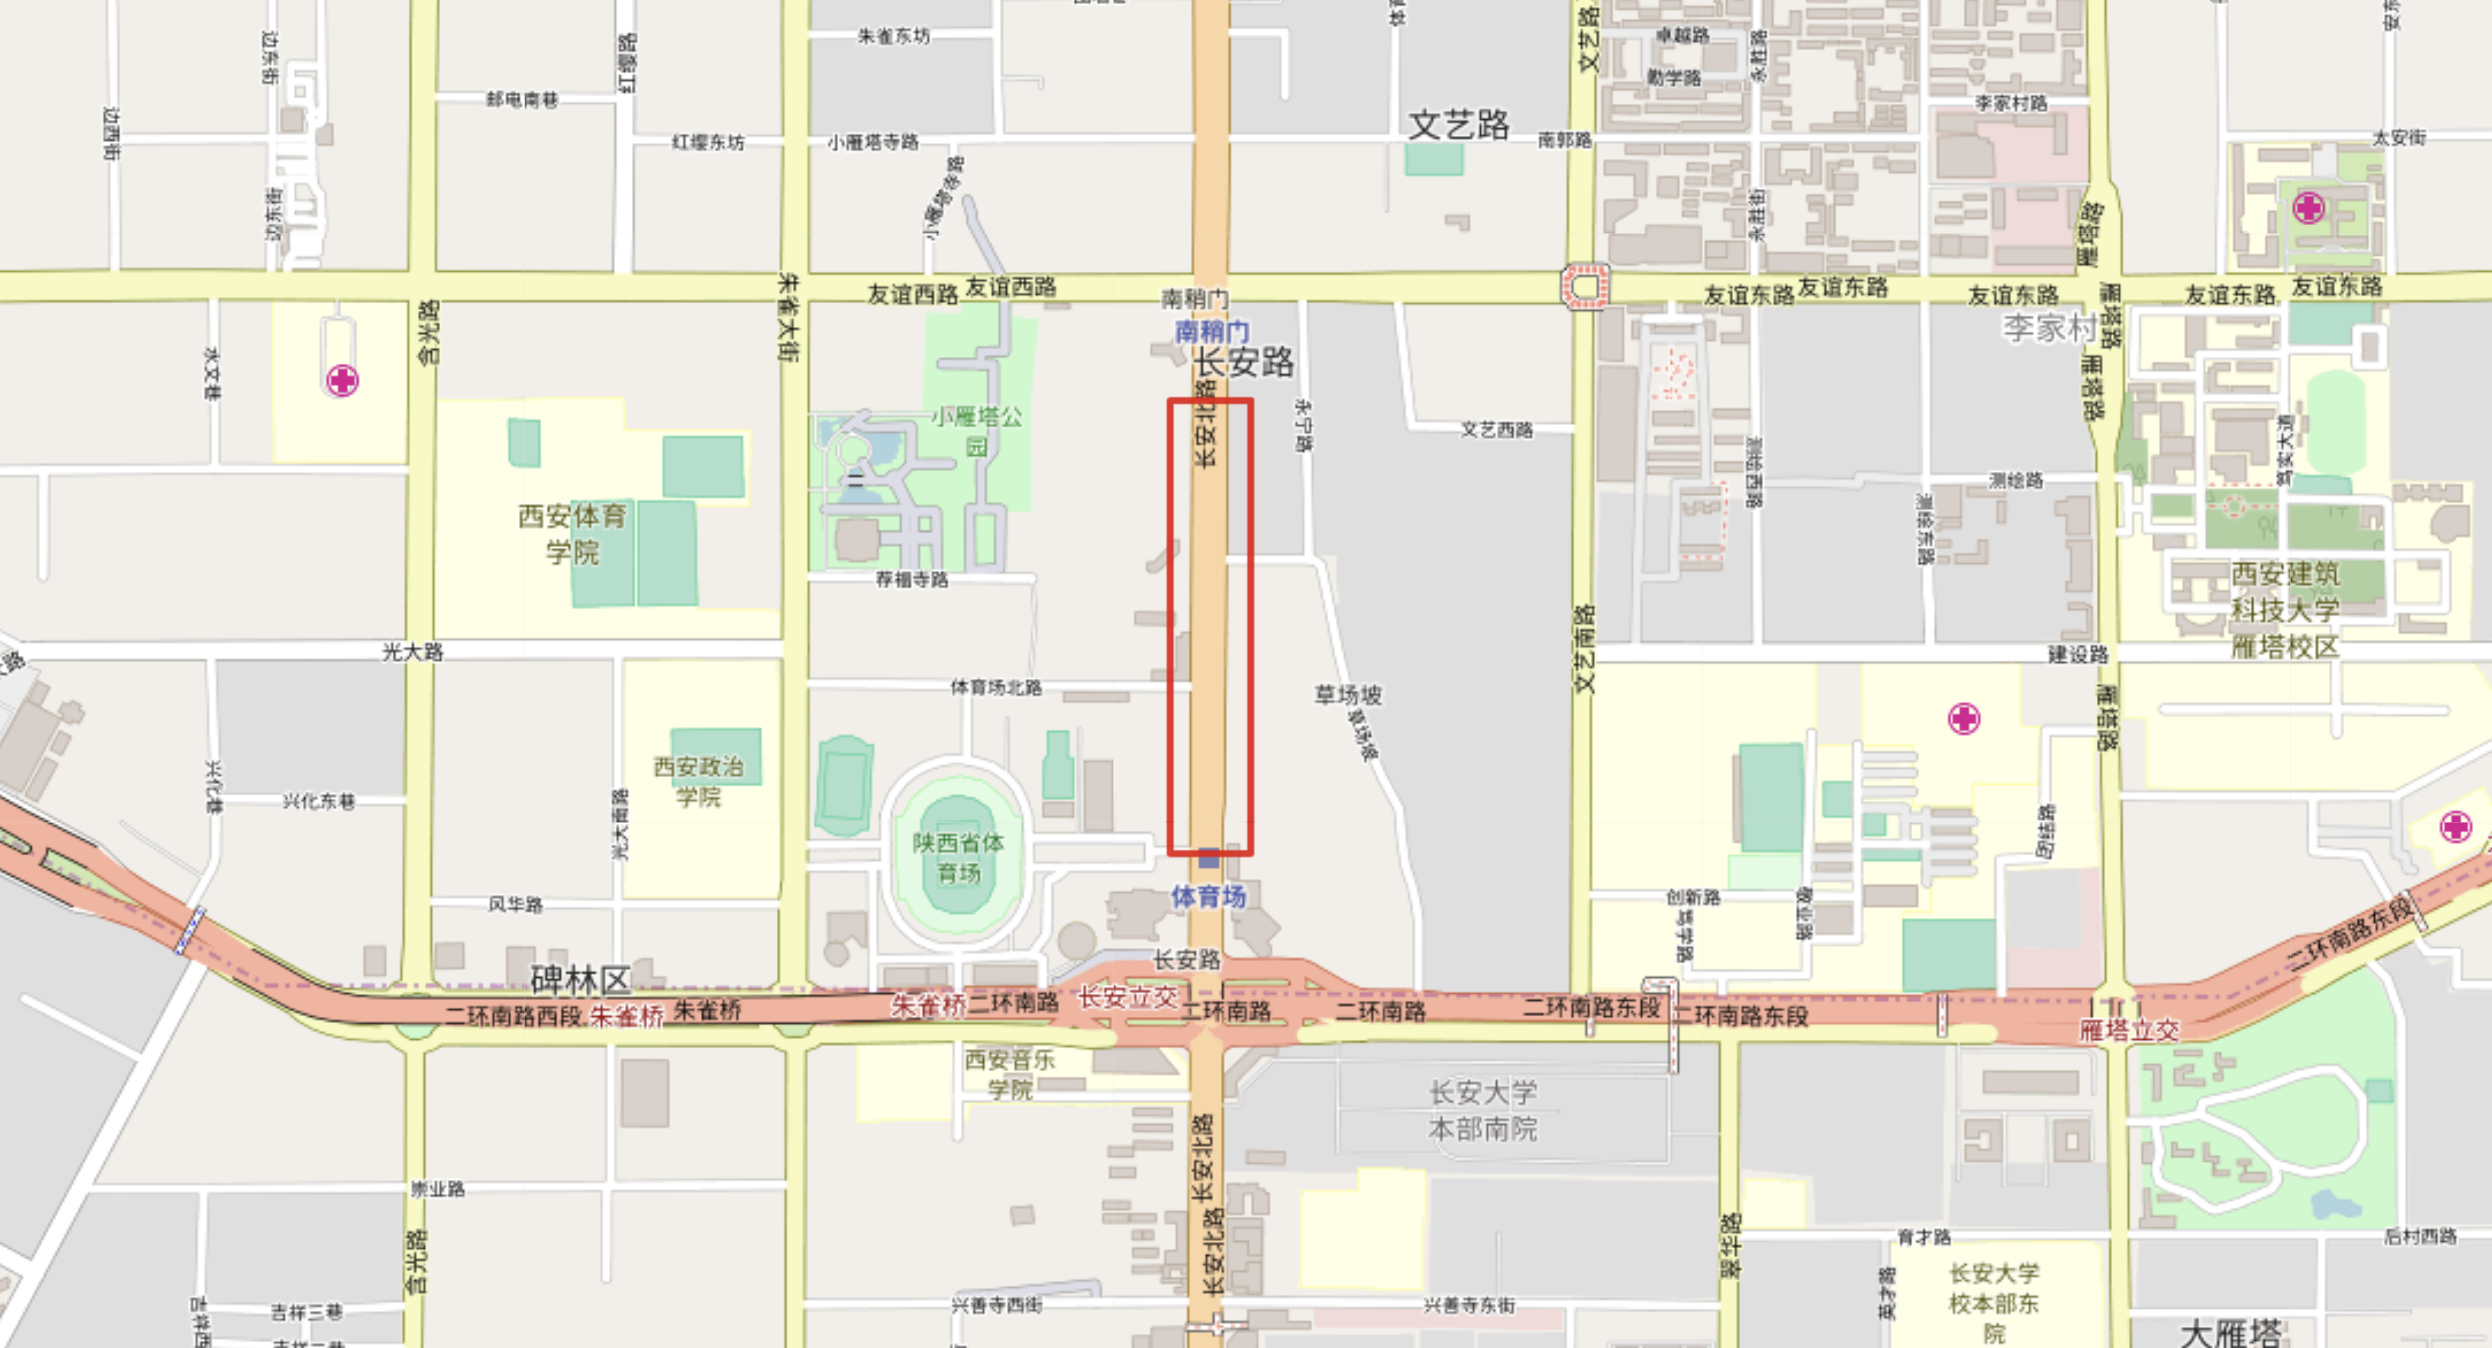
\includegraphics[width=\textwidth]{figs/XiAn}
\end{minipage}
\begin{minipage}{0.45\linewidth}
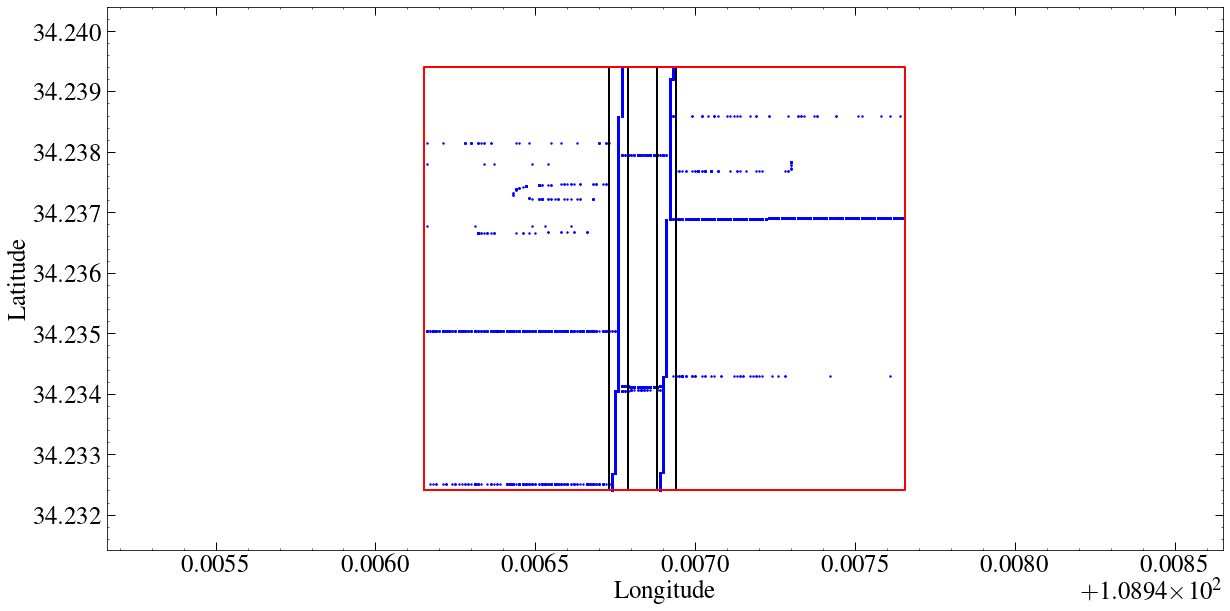
\includegraphics[width=\textwidth]{figs/lnglat}
\end{minipage}
\caption{Road section to be predict} 
\label{fig:roadsection}
\end{figure}

The road section in question is shown in red rectangular in Fig.~\ref{fig:roadsection}, and we manually locate the ranges of both north-bounding and south-bounding road sections in terms of longitudes and latitudes. We extract all trips that go through south-or-north bounding corridor. Then, from the truncated trajectory, we calculate the vehicle speed with the travel distance calculated from location information and the travel time. The speeds contain noisy data since the travel time of two sequential points is very short, approximately 2-4 seconds. The noise can be ignored in our computation, since the extracted data is sufficiently large. Another aspect is the time slots. The time offsets are split into evenly distributed cells, e.g. north-bounding time slots is a simple sequence $5, 305, 605,\ldots$, while south-bounding time slots are $4, 304, 604, \ldots$, with a gap of 5 minutes (300 seconds). Each estimated speed is allocated to its nearest time slot, e.g. the speed $k=39$ of a truncated trip $a\to b$ during $t_1=505$ and $t_2=508$, since $t_2-t_1\ll 300$, it's nature to assume that the average driving speed at the nearest time slot $t=605$ tends to be close to what at either $t_1$ or $t_2$.

\subsection*{Methods and Results}
Speed prediction is a classical regression problem. Partially based on real life facts, we assume that the future traffic speed is predictable with the historical data. The dataset is built as follows. Based on the evenly distributed time slots, we extract all speed estimations in each time slot, and the average value is assigned to the corresponding time slot. We apply the same strategy to process the trajectory data of each day. Finally, we create a dataset of size $n\times d$, with $n=284$ instance for north-bounding and $n=279$ for south-bounding traffic flow, and $d=59$ equals to the number of effective days (\textcolor{red}{Note: Oct 30 and Oct 31, 2016 are redundant copies and thrown away}). The number of instances is determined by the number of time slots, which are split following the same criterion used in the observation records.

\begin{table}[H]
\centering
\caption{Optimal hyper-parameters of models. Training rmse is the average rmse of 10 fold cross validation over the training set, which accounts for 80\% of the entire dataset, and testing rmse is over the remaining 20\% instances. The rmse corresponds to the entire dataset without the missing entries of the learned model.}
\label{tbl:params}
\begin{tabular}{c|c|c|c|c|c|c|}
\hlinew{1pt}
\multirow{2}{*}[0.1em]{South/North} & \multicolumn{3}{c|}{Random Forest} & \multirow{2}{*}[0.1em]{\textrm{train rmse}} & \multirow{2}{*}[0.1em]{\textrm{test rmse}} & \multirow{2}{*}[0.1em]{\textrm{rmse}}\\
\cline{2-4}
 & n\_estimators & max\_depth & & &&\\
\hline
South & 200 & 4 && 2.358 & 6.016 & 4.140\\
\hline
North & 100 & 4 && 4.195 & 9.915 & 7.036\\
\hlinew{1pt}
\multirow{2}{*}[0.1em]{S/N} & \multicolumn{3}{c|}{Gradient Boosting} & \multirow{2}{*}[0.1em]{\textrm{train rmse}} & \multirow{2}{*}[0.1em]{\textrm{test rmse}} & \multirow{2}{*}[0.1em]{\textrm{rmse}}\\
\cline{2-4}
 & n\_estimators & max\_depth & learning\_rate &&&  \\
\hline
South & 60 & 3 & 0.184 & 0.084 & 6.750 & 2.950\\
\hline
North & 240 & 2 & 0.109 & 0.548 & 9.409 & 4.646\\
\hlinew{1pt}
\multirow{2}{*}[0.1em]{S/N} & \multicolumn{3}{c|}{SVR (RBF kernel)} & \multirow{2}{*}[0.1em]{\textrm{train rmse}} & \multirow{2}{*}[0.1em]{\textrm{test rmse}} & \multirow{2}{*}[0.1em]{\textrm{rmse}}\\
\cline{2-4}
 & gamma & C & epsilon & && \\
\hline
South & 0.101 & 546.870 & 0.120 & 0.119 & 6.283 & 3.122\\
\hline
North & 0.101 & 935.922 & 0.419 & 0.762 & 10.250 & 4.565\\
\hlinew{1pt}
\end{tabular}
\end{table}


Three models: gradient boosting, random forest and support vector regressor\footnote{https://scikit-learn.org/} are trained with the $z-$score normalized dataset, where dataset is split into training and testing set following 80:20 rule. Each has its own pros and cons. The former two are ensemble models, whose advantages include ease to implement and efficient to train, but may be overfitting, which can be counteracted with cross-validation. SVM models are hard to tune and expensive to train~\cite{bishop2006pattern,friedman2001elements}. But, they have a good generalization ability even with small data set. Also, each has many hyper-parameters to tune. Therefore, we employed the hyper-optimization method~\cite{snoek2012practical} implemented in hyperopt\footnote{https://github.com/hyperopt/}. The optimal hyper-parameters for each model are reported in \textbf{Table}~\ref{tbl:params}. With the selected model, predictions are made over the missing time periods and Fig.~\ref{fig:preds} shows the snapshots of the predictions. More detailed information can be found in the attached Jupyter Notebook.

\begin{figure}[!h]
\centering
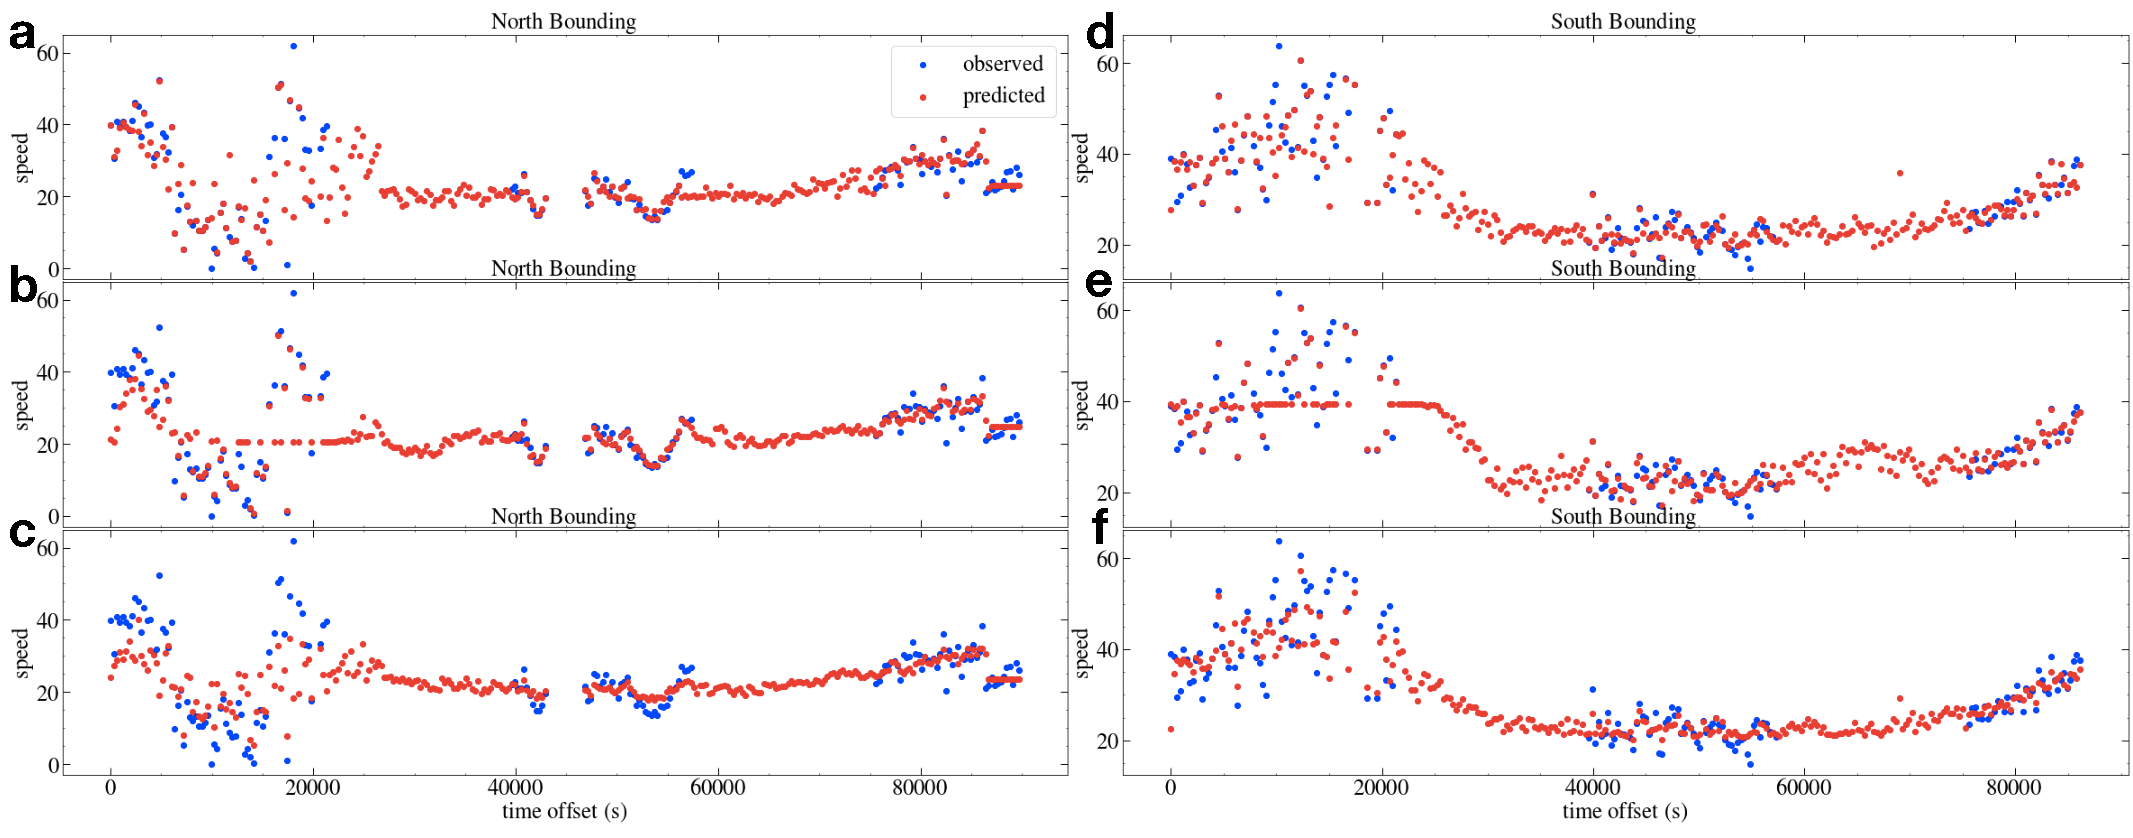
\includegraphics[width=0.8\textwidth]{figs/predictions}
\caption{\textbf{Traffic speed prediction.} \textbf{a-c,} Speed prediction on northbound, and \textbf{d-f,} on southbound corridor. \textbf{a,d} gradient boosting, \textbf{b,e} support vector, and \textbf{c,f} random forest regressor.} 
\label{fig:preds}
\end{figure}

%\begin{figure}[!h]
%\centering
%\begin{minipage}{0.48\linewidth}
%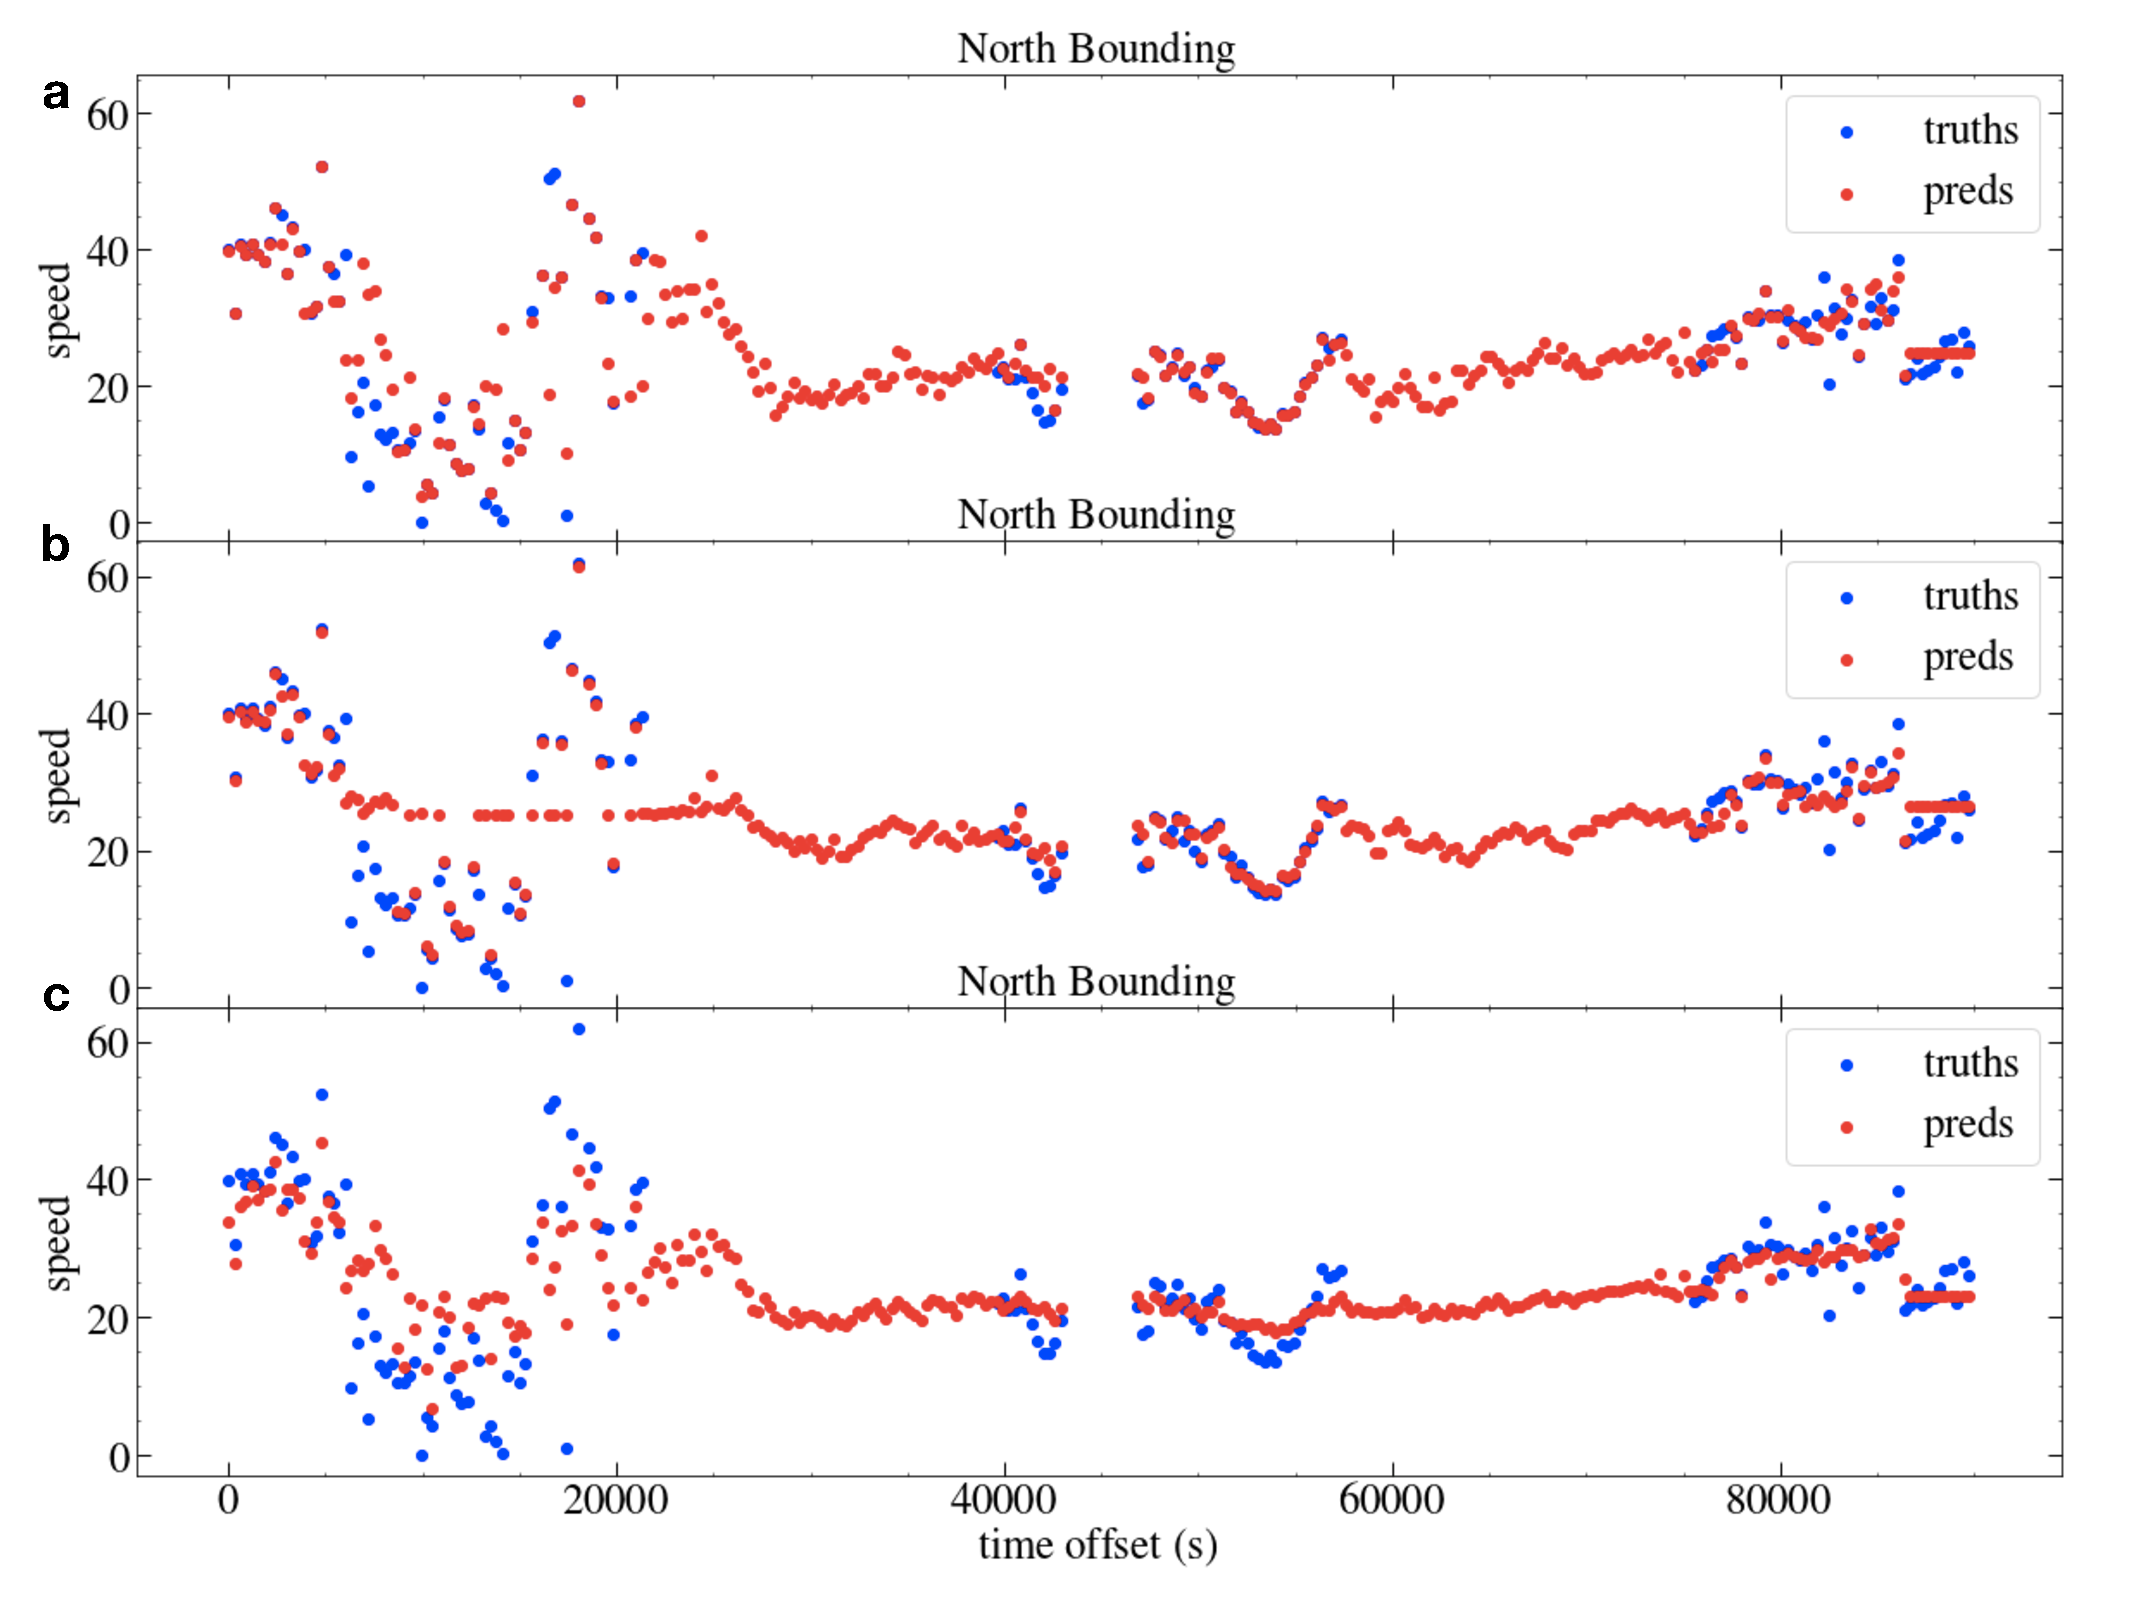
\includegraphics[width=\textwidth]{figs/north}
%\end{minipage}
%\begin{minipage}{0.48\linewidth}
%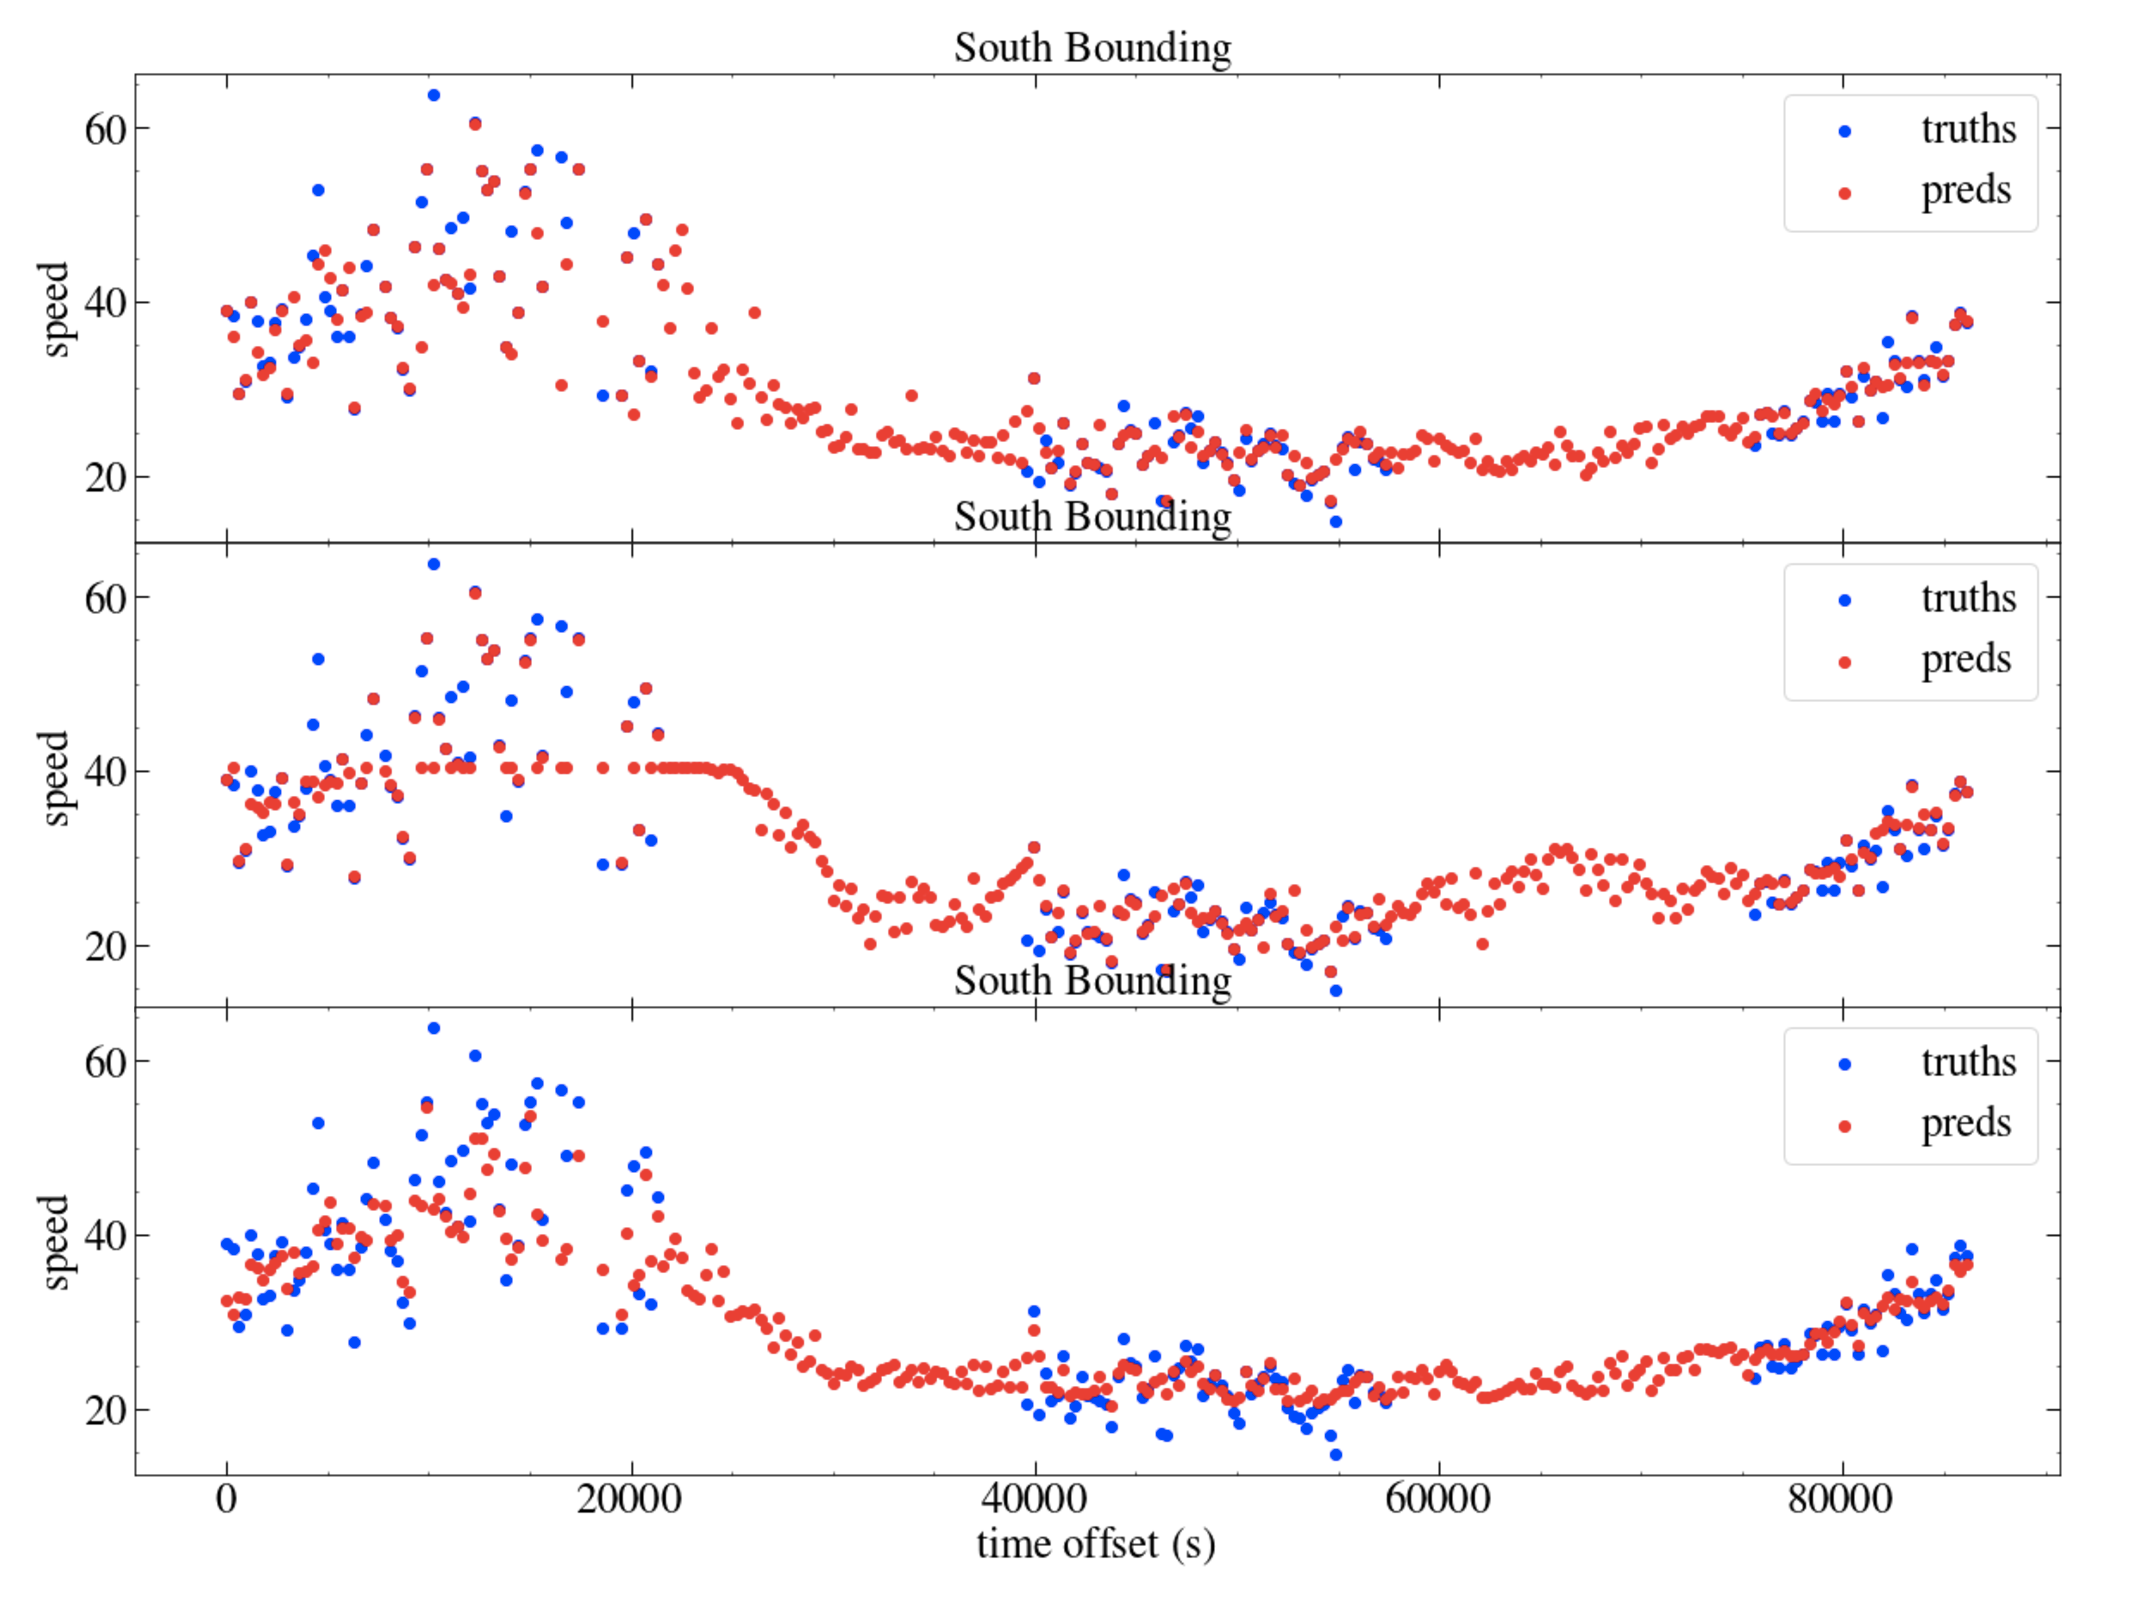
\includegraphics[width=\textwidth]{figs/south}
%\end{minipage}
%\caption{\textbf{Traffic speed prediction.} \textbf{a-c,} Speed prediction on northbound, and \textbf{d-f,} on southbound corridor. \textbf{a,d} gradient boosting, \textbf{b,e} support vector, and \textbf{c,f} random forest regressor.} 
%\label{fig:preds}
%\end{figure}

\subsection*{Discussions}
The trajectory date is sparse, especially for the given road sections. All our computations is simplified, and the created dataset does not consider other factors that exercise some extend impacts on the traffic speed, locally or globally~\cite{woodard2017predicting}, e.g. the drivers' behaviors (the size of unique drivers is found in million, many drivers may be given multiple encoding strings), the weather (snowing slows down the entire system), surrounding business (determines the demand and supply), and the entering and exiting ramps (merge/branch the traffic flow, and form bottlenecks, may cause traffic collisions). More advanced techniques can be applied, including HMM~\cite{friedman2001elements}, MCMC~\cite{woodard2017predicting} and deep neural networks~\cite{goodfellow2016deep}.

\bibliographystyle{naturemag}
\bibliography{ref}

\end{document}
